\documentclass[CMPE]{KGCOEReport}

\usepackage{graphicx}
\usepackage{newtxtext, newtxmath}
\usepackage{csquotes}
\usepackage{parskip}
\usepackage{karnaugh-map}
\usepackage{float}
\usepackage{hyperref}
\usepackage[super]{nth}
\usepackage{pdfpages}

\graphicspath{{./assets/}}

\newcommand{\classCode}{CMPE 260}
\newcommand{\name}{Aden Perry}
\newcommand{\LabSectionNum}{L2}
\newcommand{\LabInstructor}{Richard Cliver}

\newcommand{\TAs}{Eric Reed \\ Tevin Hendess}
\newcommand{\LectureSectionNum}{01}
\newcommand{\LectureInstructor}{Cory Merkel}
\newcommand{\exerciseNumber}{3}
\newcommand{\exerciseDescription}{Instruction Fetch and Decode Stages}
\newcommand{\dateDone}{2026-02-24}
\newcommand{\dateSubmitted}{2026-03-02}

\begin{document}

\maketitle

\section*{Abstract}
\addcontentsline{toc}{section}{Abstract}

The purpose of this exercise was to design and implement components to hold,
fetch, and decode 32-bit instructions. A byte-addressable instruction memory
module was designed to store 1024 bytes of 32-bit instructions. An instruction
fetch module was designed to fetch instructions in sequence every clock cycle by
using the memory module. A control unit was designed to decode the
\texttt{opcode} and \texttt{funct} bits of an instruction to determine which
action would be taken by the ALU, and which resources were required for that
action. An instruction decode module was designed to decode 32-bit instructions
into an ALU code, register addresses, a sign-extended immediate, and various
flags indicating required resource usage using the control unit and a
previously designed register file. The fetch and decode modules were
independently tested against different test benches. Test benches used mock
write data, as the ALU was not connected. All tests passed; the exercise was
successful.

\section*{Design Methodology}
\addcontentsline{toc}{section}{Design Methodology}

The instruction memory module took in a 28-bit address and output the
corresponding 32-bit instruction. Only 1024 bytes could be stored; any input
address outside the storage range simply output the byte \texttt{0x00}. The
memory was byte addressable, and returned the addressed byte as well as the
following three bytes. On the edges of the storage range (the \nth{1024},
\nth{1023}, and \nth{1021} bytes), the stored bytes were concatenated with
\texttt{0x00}. Memory was initialized with signal default assignment. It is
impossible to change the values in instruction memory without editing and
recompiling the VHDL specification.

The instruction fetch module took a clock and an asynchronous active-high reset
as inputs, and gave a 32-bit instruction as output. It maintained a program
counter which incremented by four every clock cycle. On reset, the program
counter was set to 0. The instruction memory module was instantiated as a
component for the fetch module. The program counter was used as an input
address to the instruction memory module. The output of the instruction memory
module was mapped directly to the output of the instruction fetch module.


\begin{table}[H]

	% Introduction has to be on same page
	The control unit took in a 6-bit \texttt{opcode} and \texttt{funct} and
	output the ALU code for the relevant operation as well as flags indicating
	whether registers would be modified, memory would be modified, memory would
	be written to, and two flags indicating whether an immediate number would
	be used. All outputs were determined using if-then and with-select
	statements; thus, the control unit must be compiled with support for VHDL
	2008 or higher. Each output was assigned inside a seperate process for
	better code seperation and readability. If the \texttt{opcode} was all
	zeroes, the instruction did not use an immediate, and \texttt{funct} was
	used to determine the specific ALU codes. All \texttt{funct} codes and
	their corresponding instructions are given in Table \ref{tab:funct}.

	\center
	\caption{\texttt{funct} Correspondence to ALU Codes}
	\begin{tabular}{|c|c|c|}
		\hline
		\texttt{funct} & ALU Code & Function \\
		\hline
		\hline
		100000         & 0100     & ADD      \\
		\hline
		100100         & 1010     & AND      \\
		\hline
		011001         & 0110     & MULTU    \\
		\hline
		100101         & 1000     & OR       \\
		\hline
		000000         & 1100     & SLL      \\
		\hline
		000011         & 1110     & SRA      \\
		\hline
		000010         & 1101     & SRL      \\
		\hline
		100010         & 0101     & SUB      \\
		\hline
		100110         & 1011     & XOR      \\
		\hline
	\end{tabular}
	\label{tab:funct}
\end{table}

\begin{table}[H]

	If the \texttt{opcode} code was not all zeroes, the instruction used an
	immediate, and \texttt{opcode} was used to determine the specific ALU
	codes. All \texttt{opcode} codes and their corresponding ALU instructions
	are given in Table \ref{tab:opcode}.

	% Introduction has to be on same page
	\center
	\caption{\texttt{opcode} Correspondence to ALU Codes}
	\begin{tabular}{|c|c|c|}
		\hline
		\texttt{opcode} & ALU Code & Function \\
		\hline
		\hline
		001000          & 0100     & ADDI     \\
		\hline
		001100          & 1010     & ANDI     \\
		\hline
		001101          & 1000     & ORI      \\
		\hline
		001110          & 1011     & XORI     \\
		\hline
		101011          & 0100     & SW       \\
		\hline
		100011          & 0100     & LW       \\
		\hline
	\end{tabular}
	\label{tab:opcode}
\end{table}

If the \texttt{opcode} code was not all zeroes and the \texttt{funct} did not
match one of the codes given in Table \ref{tab:funct}, or else if the
\texttt{opcode} code did not match one of those given in Table
\ref{tab:opcode}, an invalid instruction was specified and an ALU code of 1100
was assumed.

The instruction decode module took as inputs a 32-bit instruction, a 5-bit
register write address, a 32-bit register write data, and a 1-bit register
write enable. It gave as outputs 1-bit flags indicating whether the instruction
required a register write, a memory read, a memory write, and 2 flags
indicating whether an immediate was used. It also gave a 4-bit ALU control
code, two 32-bit register data reads, two 32-bit register write addresses, and
one sign-extended 32-bit immediate number. A control unit was instantiated.
Bits 32--26 were assigned as the \texttt{opcode} for the control unit. Bits
5--0 were assinged as the \texttt{funct}. Output flags from the control unit
were assigned to output flags for the decode module. A register file was
instantiated. Bits 25--21 and bits 20--16 were assigned as read addresses. The
inputs write address, write data, and write enable were assigned as the write
address, write data, and write enable for the register file, respectively. The
output register reads were assigned as the decode module output register reads.
Bits 15--0 of the instruction were sign-extended and assigned to the 32-bit
immediate out. All outputs were asynchronous except for the register reads. A
process statement was used to sign-extend the immediate; all other outputs
were simple one-liners.

Instruction fetch and instruction decode were not connected in any way in this
exercise. However, in future exercises, the instruction input for the decode
module will come from the instruction output from the fetch module.

\section*{Results and Analysis}
\addcontentsline{toc}{section}{Results and Analysis}

In order to verify the correctness of the instruction fetch module, a test
bench was created containing 9 tests. Tests were chosen to ensure basic
functionality: reset, and that sequential 4-byte instructions are returned. The
edge cases of out-of-bounds instruction access and unalgined instruction access
are not tested; the former because it would take hundreds of test clock cycles,
and the latter because it is physically impossible to get an unalgined acces
while only providing stimuli to the instruction fetch module. The waveform
generated by a behavioral simulation against the test bench is given in Figure
\ref{fig:fetch-behv}.

\begin{figure}[H]
    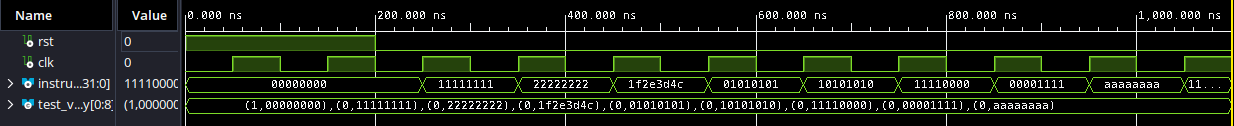
\includegraphics[width=\textwidth]{fetch-behv}
    \caption{Waveform for Behavioral Testbench of Instruction Fetch}
    \label{fig:fetch-behv}
\end{figure}

The waveform shown in Figure \ref{fig:fetch-behv} shows that the design was
implemented correctly.

For example, the reset functionality was tested between 0 ns and 200 ns, as
shown in Figure \ref{fig:fetch-behv-1}

\begin{figure}[H]
    \center
    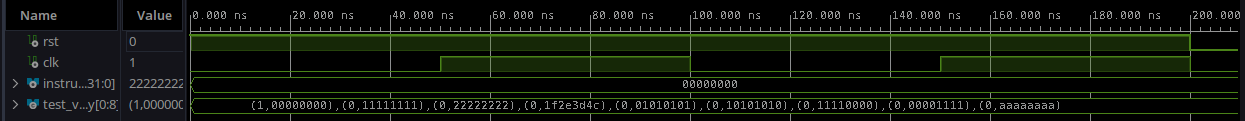
\includegraphics[width=\textwidth]{fetch-behv-1}
    \caption{Waveform for Reset Fetch Test}
    \label{fig:fetch-behv-1}
\end{figure}

The waveform given in Figure \ref{fig:fetch-behv-1} shows a reset being sent to
the instruction fetch module, and the instruction being set to
\texttt{0x00000000}, the first instruction. This is the correct behavior for
the reset operation; the test passed.

\pagebreak

The instruction fetch functionality was tested between 200 ns and 400 ns, as
shown in Figure \ref{fig:fetch-behv-2}.

\begin{figure}[H]
    \center
    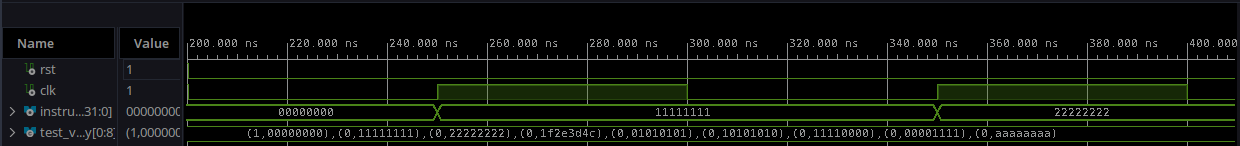
\includegraphics[width=\textwidth]{fetch-behv-2}
    \caption{Waveform for Instruction Fetch Test}
    \label{fig:fetch-behv-2}
\end{figure}

The waveform given in Figure \ref{fig:fetch-behv-2} shows an instruction being
fetched from the instruction fetch module, and the instructions
\texttt{0x11111111} and \texttt{0x22222222} being fetched. These are the second
and third instructions in the instruction memory module.
This is the correct behavior for the instruction fetch operation; the test
passed.

The instruction fetch functionality was further tested between 400 ns and 600
ns, as shown in Figure \ref{fig:fetch-behv-3}.

\begin{figure}[H]
    \center
    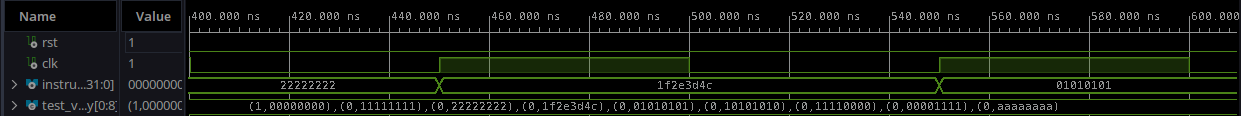
\includegraphics[width=\textwidth]{fetch-behv-3}
    \caption{Waveform for Second Instruction Fetch Test}
    \label{fig:fetch-behv-3}
\end{figure}

The waveform given in Figure \ref{fig:fetch-behv-3} shows an instruction being
fetched from the instruction fetch module, and the instructions
\texttt{0x1f2e3d4c} and \texttt{0x01010101} being fetched. These are the fourth
and fifth instructions in the instruction memory module.
This is the correct behavior for the instruction fetch operation; the test
passed.

The instruction fetch module was also tested using a post-implementation
simulation to simulate exact timings. The testbench for the entire
post-implementation timing simulation is given in Figure \ref{fig:fetch-pimp}.

\begin{figure}[H]
    \center
    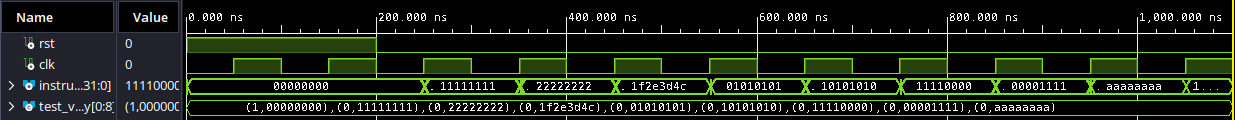
\includegraphics[width=\textwidth]{fetch-pimp}
    \caption{Waveform for Post-Implementation Testbench of Instruction Fetch}
    \label{fig:fetch-pimp}
\end{figure}

The waveform given in Figure \ref{fig:fetch-pimp} shows that the design would
work if implemented in hardware. It shows the required time to wait after an
input change before an output signal can be trusted.

\pagebreak

For example, the same reset function tested in Figure \ref{fig:fetch-behv-1}
is tested with post-implementation timing. The waveform is given in Figure
\ref{fig:fetch-pimp-1}.

\begin{figure}[H]
    \center
    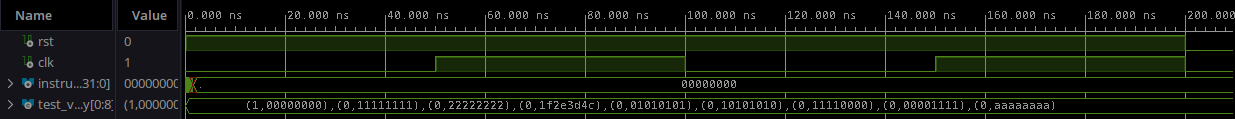
\includegraphics[width=\textwidth]{fetch-pimp-1}
    \caption{Waveform for Reset Post-Implementation Test Fetch}
    \label{fig:fetch-pimp-1}
\end{figure}

The waveform given in Figure \ref{fig:fetch-pimp-1} shows that the reset
functionality works as expected and that a small delay of approximately 2 ns
must occur before the instruction output can be trusted. Examining Figure
\ref{fig:fetch-pimp} and Figure \ref{fig:fetch-behv} shows that no
functionality was lost in the implementation stage of simulation. Examining
Figure \ref{fig:fetch-pimp} and \ref{fig:fetch-pimp-1} shows that a maximum of
2 ns must pass before the instruction output can be trusted.

The testbench was simulated through ModelSim to test for errors or
irregularities not caught by the Vivado simulator. The waveform of the ModelSim
testbench simulation is given in Figure \ref{fig:fetch-msim}.

\begin{figure}[H]
    \center
    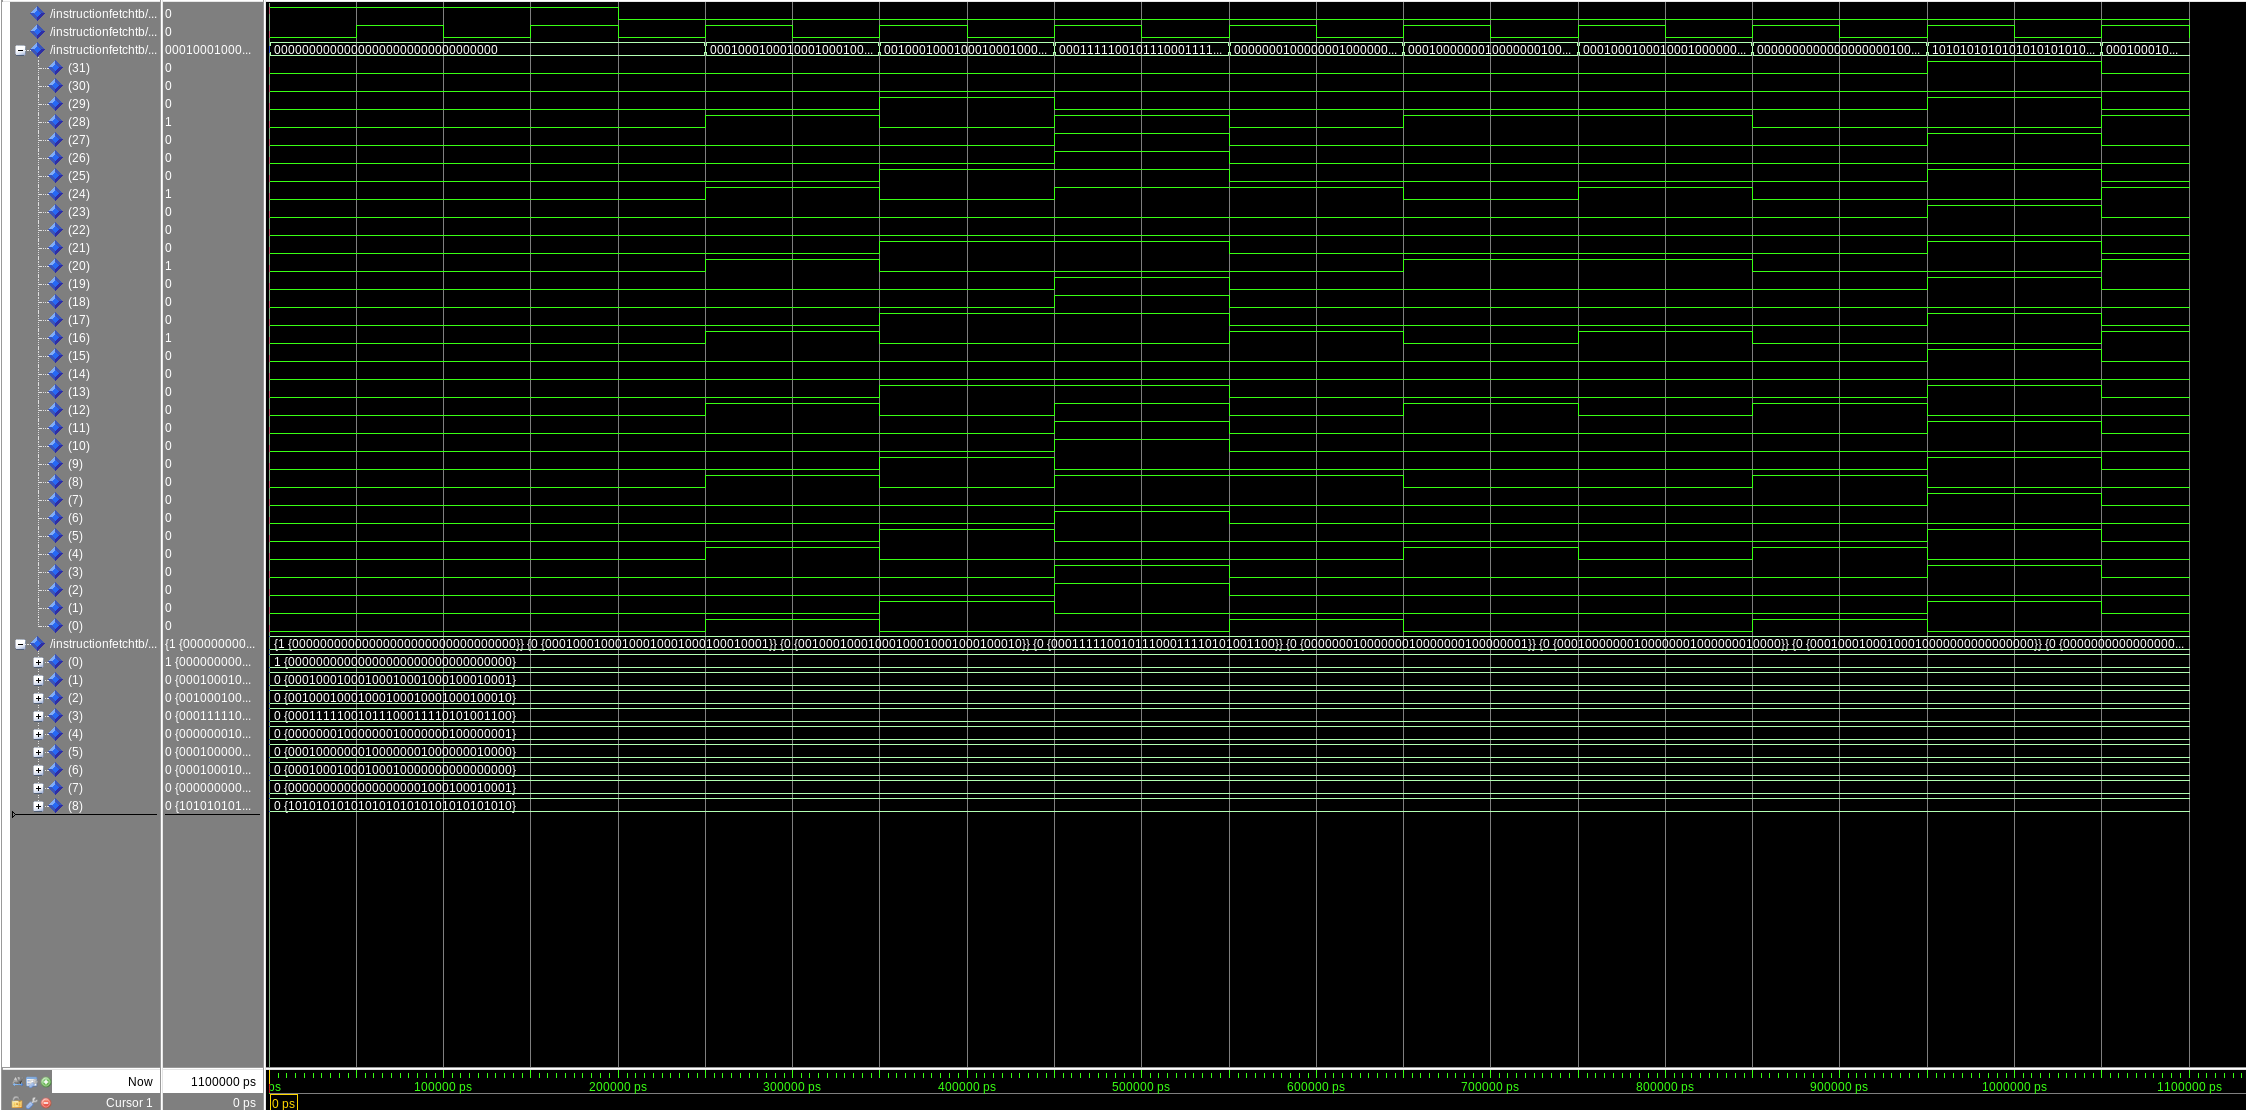
\includegraphics[width=\textwidth]{fetch-msim}
    \caption{Waveform for ModelSim Instruction Fetch Testbench}
    \label{fig:fetch-msim}
\end{figure}

The waveform given in Figure \ref{fig:fetch-msim} shows no differences compared
to the behavioral waveform given in Figure \ref{fig:fetch-behv}. Therefore,
ModelSim did not reveal any irregularities that Vivado did not.

\pagebreak
% Instruction decode section

In order to verify the correctness of the instruction decode module, a test
bench was created containing 5 tests. Tests were chosen to ensure basic
functionality: ALU decode, register reads register writes, and flag sets. Only
5 tests were made because each test contains a large quantity of inputs and
outputs. The waveform generated by a behavioral simulation against the test
bench is given in Figure \ref{fig:decode-behv}.

\begin{figure}[H]
    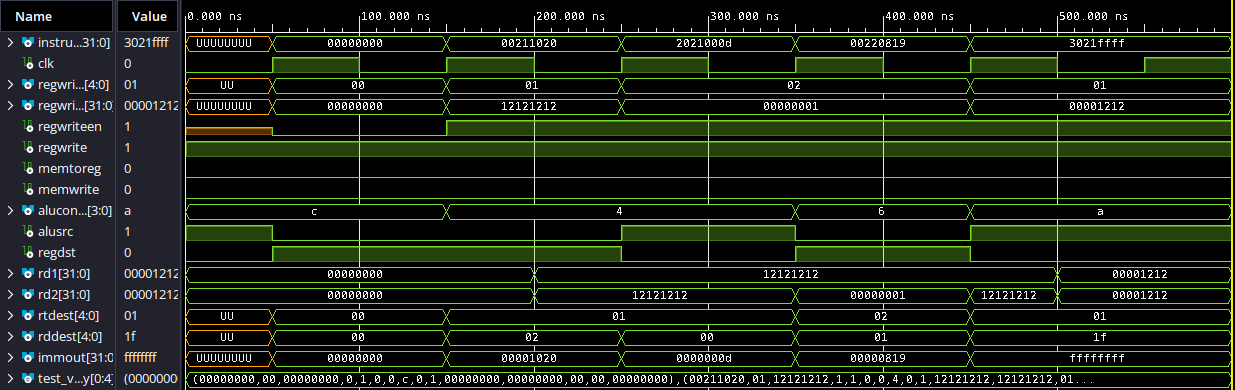
\includegraphics[width=\textwidth]{decode-behv}
    \caption{Waveform for Behavioral Testbench of Instruction Decode}
    \label{fig:decode-behv}
\end{figure}

The waveform shown in Figure \ref{fig:decode-behv} shows that the design was
implemented correctly.

For example, the initialization functionality was tested between 0 ns and 100
ns, as shown in Figure \ref{fig:decode-behv-1}.

\begin{figure}[H]
    \center
    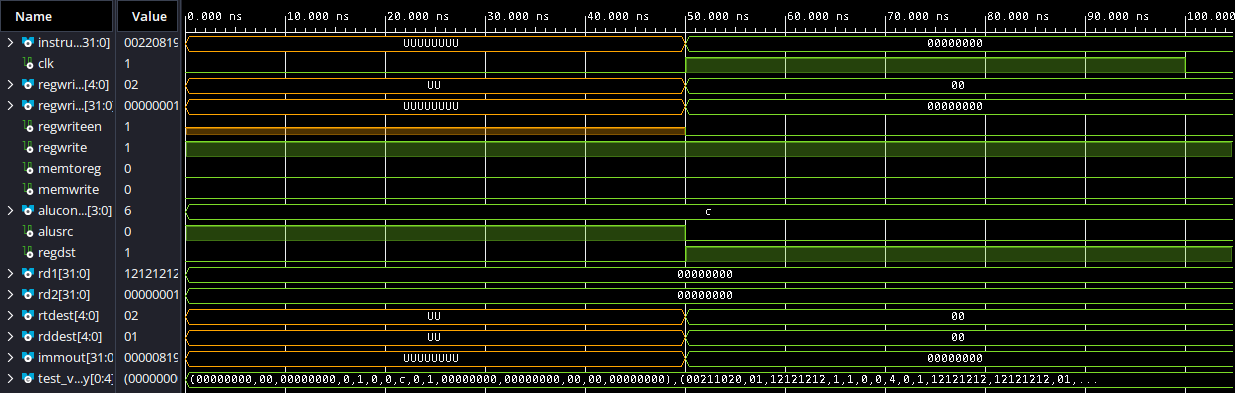
\includegraphics[width=\textwidth]{decode-behv-1}
    \caption{Waveform for Initialization Decode Test}
    \label{fig:decode-behv-1}
\end{figure}

The waveform given in Figure \ref{fig:decode-behv-1} shows an initial value of
zeroes being assigned to every input on the clock edge, and all outputs being
initialized.
This is the correct behavior for the reset operation; the test passed.

\pagebreak

An R-type instruction was tested between 100 ns and 200 ns,
as shown in Figure \ref{fig:decode-behv-2}.

\begin{figure}[H]
    \center
    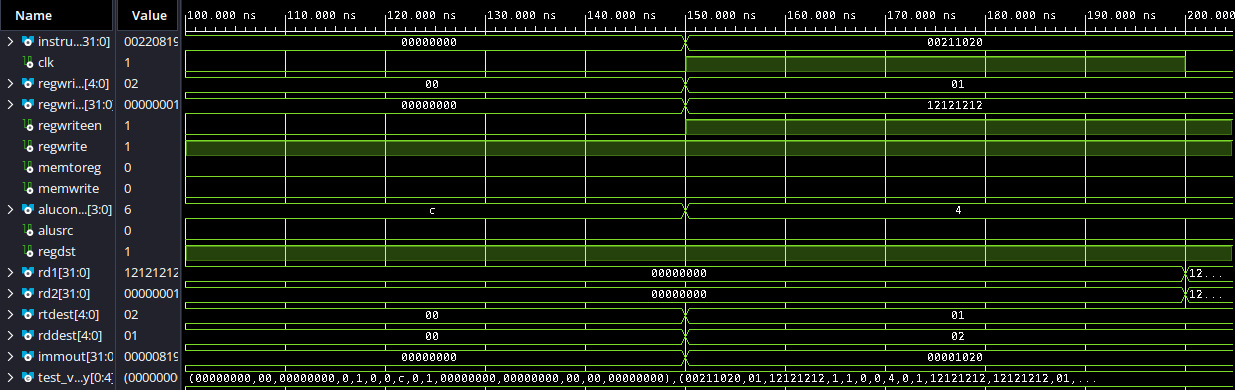
\includegraphics[width=\textwidth]{decode-behv-2}
    \caption{Waveform for R-Type Instruction Decode Test}
    \label{fig:decode-behv-2}
\end{figure}

The waveform given in Figure \ref{fig:decode-behv-2} shows
an \texttt{opcode} of zeroes and a \texttt{funct} of \texttt{100000}. It also
shows register write data of \texttt{0x12121212} to register address 1. The ALU
code was decoded to \texttt{0100}. The read data from register address 1 showed
the write data. Flags indicated that an immediate was not used.
This is the correct behavior for the R-type instruction decode operation; the
test passed.

An I-type instruction was tested between 200 ns and 300 ns,
as shown in Figure \ref{fig:decode-behv-3}.

\begin{figure}[H]
    \center
    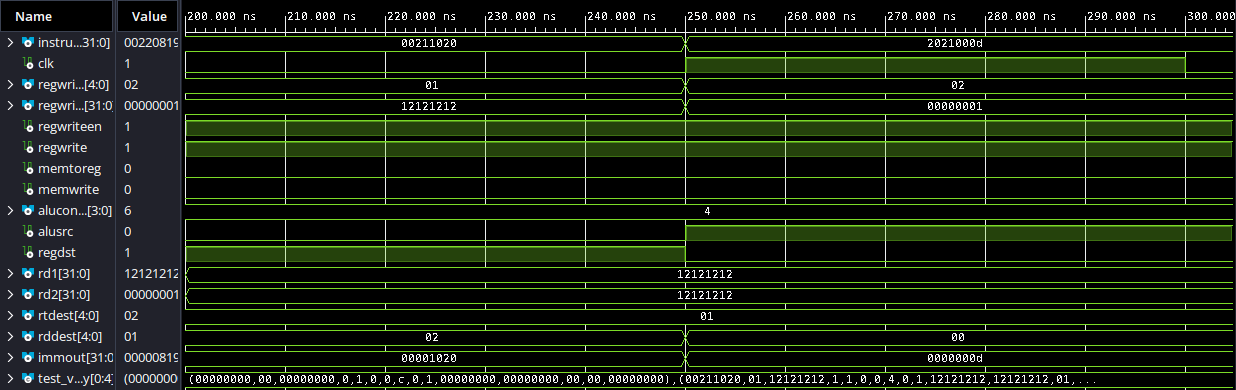
\includegraphics[width=\textwidth]{decode-behv-3}
    \caption{Waveform for I-Type Instruction Decode Test}
    \label{fig:decode-behv-3}
\end{figure}

The waveform given in Figure \ref{fig:decode-behv-3} shows
an \texttt{opcode} of \texttt{001000} and bits 15--0 of \texttt{0x000D}. The
ALU code was decoded to \texttt{0100}. The 32-bit immediate out was
sign-extended to \texttt{0x0000000D}.
This is the correct behavior for the I-type instruction decode operation; the
test passed.

\pagebreak

The instruction decode module was also tested using a post-implementation
simulation to simulate exact timings. The testbench for the entire
post-implementation timing simulation is given in Figure \ref{fig:decode-pimp}.

\begin{figure}[H]
    \center
    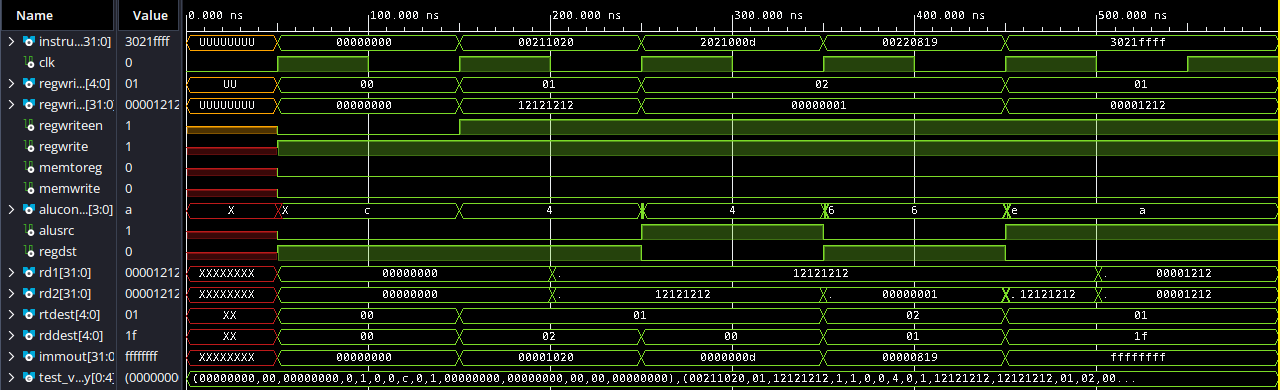
\includegraphics[width=\textwidth]{decode-pimp}
    \caption{Waveform for Post-Implementation Testbench of Instruction Decode}
    \label{fig:decode-pimp}
\end{figure}

The waveform given in Figure \ref{fig:decode-pimp} shows that the design would
work if implemented in hardware. It shows the required time to wait after an
input change before an output signal can be trusted.

For example, the same I-type instruction tested in Figure \ref{fig:decode-behv-3}
is tested with post-implementation timing. The waveform is given in Figure
\ref{fig:decode-pimp-3}.

\begin{figure}[H]
    \center
    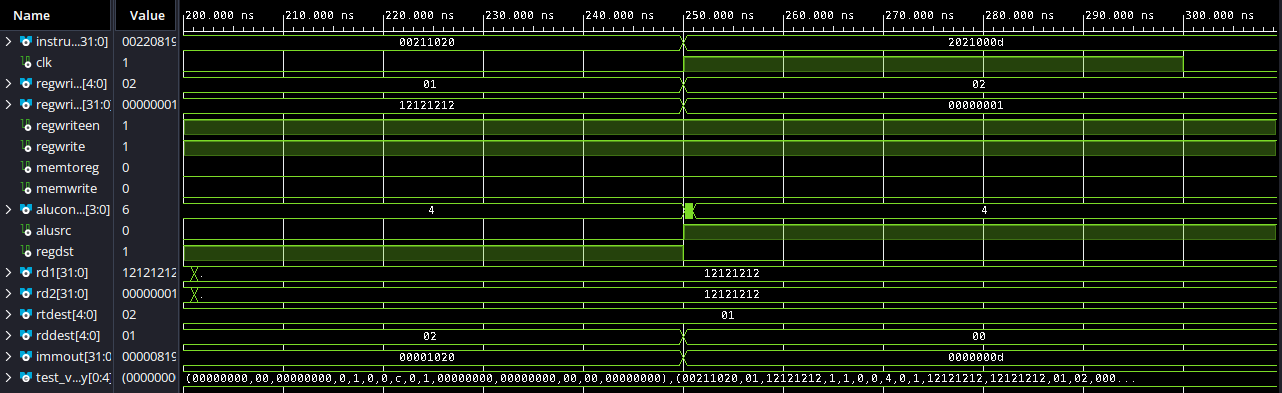
\includegraphics[width=\textwidth]{decode-pimp-3}
    \caption{Waveform for I-Type Instruction Post-Implementation Test Decode}
    \label{fig:decode-pimp-3}
\end{figure}

The waveform given in Figure \ref{fig:decode-pimp-3} shows that the reset
functionality works as expected and that a small delay of approximately 1 ns
must occur before the instruction output can be trusted. Examining Figure
\ref{fig:decode-pimp} and Figure \ref{fig:decode-behv} shows that no
functionality was lost in the implementation stage of simulation. Examining
Figure \ref{fig:decode-pimp} and \ref{fig:decode-pimp-3} shows that a maximum of
about 1.5 ns must pass before the instruction output can be trusted.

\section*{Conclusion}
\addcontentsline{toc}{section}{Conclusion}

The object of the exercise was to design instruction fetch and decode stages to
fetch and instruction from memory and decode an instruction into various useful
codes and flags. This was accomplished by using components to handle
instruction storage and ALU decoding. Decoding made use of if-then and
with-select statements. The exercise was successful; all test cases were
passed. Processes were shown to be useful tools in managing large components
with many outputs. Additionally, with-select statements were shown to be a
consise way of representing a bus that depends on the value of another bus. In
future exercises, both VHDL concepts will be used extensively to manage large
large projects where readability is a concern.


\includepdf[pages=-]{assets/prelab}
\end{document}
